% THIS IS AN EXAMPLE DOCUMENT FOR VLDB 2012
% based on ACM SIGPROC-SP.TEX VERSION 2.7
% Modified by  Gerald Weber <gerald@cs.auckland.ac.nz>
% Removed the requirement to include *bbl file in here. (AhmetSacan, Sep2012)
% Fixed the equation on page 3 to prevent line overflow. (AhmetSacan, Sep2012)

\documentclass{vldb}
\usepackage{graphicx}
\usepackage{balance}  % for  \balance command ON LAST PAGE  (only there!)
\usepackage{colortbl}
%\usepackage{subfig}

\begin{document}

% ****************** TITLE ****************************************

\title{Sampling from repairs of Denial Constraints}

% possible, but not really needed or used for PVLDB:
%\subtitle{[Extended Abstract]
%\titlenote{A full version of this paper is available as\textit{Author's Guide to Preparing ACM SIG Proceedings Using \LaTeX$2_\epsilon$\ and BibTeX} at \texttt{www.acm.org/eaddress.htm}}}

% ****************** AUTHORS **************************************

% You need the command \numberofauthors to handle the 'placement
% and alignment' of the authors beneath the title.
%
% For aesthetic reasons, we recommend 'three authors at a time'
% i.e. three 'name/affiliation blocks' be placed beneath the title.
%
% NOTE: You are NOT restricted in how many 'rows' of
% "name/affiliations" may appear. We just ask that you restrict
% the number of 'columns' to three.
%
% Because of the available 'opening page real-estate'
% we ask you to refrain from putting more than six authors
% (two rows with three columns) beneath the article title.
% More than six makes the first-page appear very cluttered indeed.
%
% Use the \alignauthor commands to handle the names
% and affiliations for an 'aesthetic maximum' of six authors.
% Add names, affiliations, addresses for
% the seventh etc. author(s) as the argument for the
% \additionalauthors command.
% These 'additional authors' will be output/set for you
% without further effort on your part as the last section in
% the body of your article BEFORE References or any Appendices.

\numberofauthors{1} %  in this sample file, there are a *total*
% of EIGHT authors. SIX appear on the 'first-page' (for formatting
% reasons) and the remaining two appear in the \additionalauthors section.


% You can go ahead and credit any number of authors here,
% e.g. one 'row of three' or two rows (consisting of one row of three
% and a second row of one, two or three).
%
% The command \alignauthor (no curly braces needed) should
% precede each author name, affiliation/snail-mail address and
% e-mail address. Additionally, tag each line of
% affiliation/address with \affaddr, and tag the
% e-mail address with \email.
%
% 1st. author
% 2nd. author
% 3rd. author
\author{
\alignauthor Hemant Saxena \\
	\affaddr{University of Waterloo}\\
	\email{h2saxena@uwaterloo.ca}
}

% There's nothing stopping you putting the seventh, eighth, etc.
% author on the opening page (as the 'third row') but we ask,
% for aesthetic reasons that you place these 'additional authors'
% in the \additional authors block, viz.
%\additionalauthors{Additional authors: John Smith (The Th{\o}rv\"{a}ld Group, {\texttt{jsmith@affiliation.org}}), Julius P.~Kumquat
%(The \raggedright{Kumquat} Consortium, {\small \texttt{jpkumquat@consortium.net}}), and Ahmet Sacan (Drexel University, {\small \texttt{ahmetdevel@gmail.com}})}
%\date{30 July 1999}
% Just remember to make sure that the TOTAL number of authors
% is the number that will appear on the first page PLUS the
% number that will appear in the \additionalauthors section.


\maketitle

\begin{abstract}
Write abstract here.
\end{abstract}


\section{Introduction} \label{sec:introduction}
It has been observed that data stored in the database is not always trustworthy \cite{Redman}.
Data quality experts estimate that as much as 10\% to 20\% of the total system implementation budget of a company can be wasted due to the dirty tuples in the database.
To some US businesses it has costed 600 billion dollars each year \cite{TDWI02}.
With the increasing scale of data, the problem of maintaining data quality is becoming more challenging: 
with more number of sources, data integration becomes a weak point and can potentially introduce duplicate values, integrity constraint violating tuples and missing values.
Therefore, to maintain an state-of-the-art data warehouse it becomes essential to come up with a data cleaning system.
A typical data cleaning system is responsible of two major tasks, detecting the dirty data and correcting them in the data.
Numerous data cleaning approaches have aimed at defining the data quality rules and data cleaning algorithms for those rules (e.g. \cite{Cong,Fan,Kolahi,XuChu}.

Some of the common ways of expressing data quality rules are Functional dependencies (FDs), Conditional functional dependencies (CFDs) and Denial constraints (DCs) \cite{XuChu}.
In majority of the literature FDs and CFDs have been considered as constraints encoding semantics, and any FD and CFD violations indicate a deviation in the database semantics, hence presence of dirty data.
The idea of Denial constraints was introduced by Xu et. al. \cite{XuChuDC} and is fairly new.
Denial constraints are same as universally quantified first order logic forms, and hence are capable of expressing varied type of constraints which can involve predicates
like "\textit{greater-than}" or "\textit"{not-equal-to}" also, including FDs and CFDs.
Most of the previous data cleaning algorithms \cite{Cong,Fan,Kolahi} considered the integrity constraints in isolation while generating the repairs.
Later work by Xu et. al.\cite{XuChu} proposed a holistic data cleaning approach, that is capable of repairing all violations together using a single objective function.
Consider the example database instance given in Table \ref{tab:eg1} and the following Constraints:

\begin{enumerate}
\item[c1] : $ \neg(t_i.A = t_j.A \wedge t_i.C \neq t_j.C)$
\item[c2] : $ \neg(t_i.B = t_j.B \wedge t_i.C \neq t_j.C)$
\item[c3] : $ \neg(t_i.D = 5 \wedge t_i.C \neq 5)$
\item[c4] : $ \neg(t_i.C < t_i.D )$
\end{enumerate}

A holistic data cleaning approach can generate the following repair:
$t_1.C = t_2.C = t_3.C = t_4.C = 5$.
However, there exist numerous possible repairs for one instance of unclean database.
For example, Table \ref{tab:eg2} shows two possible repairs of data instance in Table \ref{tab:eg1}.
A cell with value "V" can be modified to several values in order to satisfy the DC.
\begin{table} \label{tab:eg1}
\centering 
\begin{tabular}{|c|c|c|c|c|}  \hline
      & A & B & C & D 	\\ \hline
   $t_1$ & 1 & 2 & 1 & 3 	\\ \hline
   $t_2$ & 1 & 1 & 2 & 1 	\\ \hline
   $t_3$ & 2 & 1 & 3 & 1 	\\ \hline
   $t_4$ & 3 & 1 & 3 & 5 	\\ \hline
\end{tabular}
\caption{Sample Data.}
\end{table}

\begin{table} \label{tab:eg2}
\centering 
\begin{tabular}{|c|c|c|c|c|}  \hline
      & A & B & C & D 	\\ \hline
   $t_1$ & 1 & 2 & \cellcolor[gray]{0.9} 5 & 3 	\\ \hline
   $t_2$ & 1 & 1 & \cellcolor[gray]{0.9} 5 & 1 	\\ \hline
   $t_3$ & 2 & 1 & \cellcolor[gray]{0.9} 5 & 1 	\\ \hline
   $t_4$ & 3 & 1 & \cellcolor[gray]{0.9} 5 & 5 	\\ \hline
\end{tabular}
\quad
\begin{tabular}{|c|c|c|c|c|}  \hline
      & A & B & C & D 	\\ \hline
   $t_1$ & 1 & 2 & \cellcolor[gray]{0.9} 3 & 3 	\\ \hline
   $t_2$ & 1 & 1 & \cellcolor[gray]{0.9} 3 & 1 	\\ \hline
   $t_3$ & 2 & 1 & 3 & 1 	\\ \hline
   $t_4$ & 3 & 1 & 3 & \cellcolor[gray]{0.9} $V \leq 3$ 	\\ \hline
\end{tabular}
\caption{Two possible repairs.}
\end{table}

In this paper, we present an approach to data repair, that is capable of generating various possible repairs from a defined set of reapir space.
One should note that number of possible repairs are exponential for a given number of cells in the data instance.
Some "unnecessary" cells can be changed which do not take part in the violation and can still be a candidate repair.
For example, in the repairs in Table \ref{tab:eg2} also change cell $t_4.A$ to 4, and it will be valid repair.
The main challenge while generating a sample repair from the space of possible repair is to generate meaningfull repairs, repairs which do not involve "unnecessary" changes.
We will now show some examples which motivate the approach of sampling from a suitable set of repairs, described in this paper.

\subsection{Motivating Examples}
The previous data repair approaches can be majorly categorized into frameworks.
One, stems on the idea of generating single, near-optimal repair, in term sof number of deletions or attribute modifications \cite{Kolahi} \cite{Bohannon}.
For example, second repair in Table \ref{tab:eg2} will be optimal as it has fewer changes.
Second approach is of consistent query answering, that computes answers to a selected classes of queries that seems to be valid in every suitable repair \cite{Arenas,Chomicki,Fuxman,Wijsen}.

The following examples show that the existing approaches are not suitable for them, and hence motivates a sampling approach described in the paper \cite{Beskales_sampling}:

\medskip

\textit{Interactive Data Cleaning} - An interactive data repair is a process where a sequence of repairs are suggested to the user as a guide.
User may change some values according to one suggestion and demands more suggestions for other unclean attributes.
For example, a user may repair tuple $t_4$ according to repair 1 in Table \ref{tab:eg2} and tuple $t_2$ according to repair 2.
Therefore, the application requires several suggested repairs from a suitable space of repairs.
Hence, generating a single repair will not help in this case, 
A consistent query approach also will not work here because, an interactive approach is not associated with a particular query.

\medskip

\textit{Data Integration} - Data integration is another scenario where user-defined constraints are required to control the data modification during integration process.
Data expert often have a prior knowledge about the sanity of the data resources and can dictate rules to trust some sources over others.
Although previous approaches \cite{Bohannon,Kolahi} assign weight to the sources depending upon their trustworthiness and penalize changing a trusted data source.
They still cannot totally prevent the modification of trusted data.

\medskip

\textit{Uncertain Query Answering} - The notion of consistent query answering can be generalized to probabilistic query answering.
Problem of generating all repairs is intractable, but a meaningful subset of possible can repairs can still be computed and will be sufficient to allow probabilistic query answering.
Again, computing a single repair or a consistent query answer is not sufficient for this application.
The Monte Carlo Database (MCDB) \cite{Jampani} is one such example.

\subsection{Challenges}
Major challenges in sampling from repairs of denial constraints are:

\begin{itemize}
\item A repair expression used in holistic approach \cite{XuChu} has exponential number of solutions.
Therefore it is important to define a meaningful space of candidate repairs.
A meaningful repair is one which involves minimal number of changes with respect to the original database.
The task of finding a repair with minimal changes for DCs and numerical values only is known to be \textit{MaxSNP}-hard problem \cite{Bertossi}.
Therefore, an approximation algorithm is needed which can compute nearly-optimal repairs within a sufficiently large subset of repairs.

\item The present holistic data cleaning approach presented in \cite{XuChu} uses a minimum vertex cover idea which is capable of generating nearly-optimal repairs, but does not gaurantee to cover all the cardinality-minimal-repairs \cite{Beskales_sampling}.
Consider the data instance given in Table \ref{tab:eg1}, the holistic data cleaning approach uses minimum vertex cover and finds out $t_1.C = t_2.C = t_3.C = t_4.C = 5$ as the solution, but repair 2 in Table \ref{tab:eg2} shows that a there exist a repair which has fewer number of changes.
Hence, holistic approach can miss out some cardinality-minimal repairs.

\item The previous work on sampling repairs \cite{Beskales_sampling} consider FDs and CFDs.
The idea of building equivalence classes is not possible for DCs, because DCs are more expressive and for predicates like "\textit{greater-than}" and "\textit{less-than}" equivalence classes cannot be defined.
\end{itemize}

\subsection{Contributions}

Our main contribution in this paper are:
\begin{itemize}
\item We first show that the minimality definitions defined in \cite{Beskales_journal} also makes sense with respect to Denial-Constraints.
For a given Instance $I$ and a set $\sum$ of DCs, the space of possible repairs can be divided into Set-Minimal, Cardinality-Set-Minimal and Cardinality-Minimal repairs.
\item We prove that the holistic data cleaning approach described in \cite{XuChu} does not gaurantee to generate Cardinality-Minimal repair and can also generate repairs which are Not-Set-Minimal.
\item We give an efficient algorithm tha can 
\end{itemize}


\section{Notation and definitions} \label{sec:notations}
Consider a database scheme of the form $S = (U, R, B)$, where $U$ is a set of database domains, $R$ is a set of database predicates or relations and $B$ is a set of finite built-in predicates.
For example, in this paper, $B = \{=, <, >, \neq, \leq, \geq, \approx\}$.
Let $Dom(A)$ be the domain of an attribute $A \in U$.
We denote by $I$ and instance of $S$ consisting of $n$ tuples.
Let $t$ be a single tuple from the instance $I$, we denote $t[A]$ or $I(t[A])$ the value of the cell of the tuple $t$ under attribute $A$.

The integrity constraints in this paper are identified by \textit{denial-constraints} over relational databases.
Denial constraints are first-order formulae of the form $ \varphi = \forall \overline{x}\neg(R_1(\overline{x_1}) \wedge ... \wedge R_n(\overline{x_n}) \wedge P_1 \wedge ... \wedge P_m)$,
where $R_i \in R$ is a relation atom, and $\overline{x} = \cup \overline{x_i}$, and each $P_i$ of the form $v_i \theta c$ or $v_i \theta v_j$, where $v_i, v_j \in \overline{x}$, $c$ is a constant,
and $\theta \in B$.
Similarity predicate $\approx$ is possitive when the edit distance between two strings is above a user-defined threshold $\delta$.
Note that sungle-tuple constraints, Functional Dependencies, Matching Dependencies and Conditional Functional Dependencies are special cases of 
unary and binary denial constraints with equality and similarity predicates.

For a given database instance $I$ of schema $S$ and a DC $\varphi$, if $I$ satisfies $\varphi$, we write $I \models \varphi$.
For a given set of DCs $\sum$, we say $I \models \sum$ if and only if $\forall \varphi \in \sum, I \models \varphi$.
A repair $I'$ of an inconsistent instance $I$ is an instance that satisfies $\sum$ and has the same set of tuple identifiers in $I$.
The values of attributes in $I'$ can be different from $I$.
Also, for attributes with infinite domains, there can be infinte number of possible repairs.
In cases of infinite domain attributes we represent the repairs using a variable that can accomodate \textit{fresh-value} for its domain.
A fresh value variable can have value from $Dom(A)/Dom^a(A)$, where $Dom^a(A)$ is the domain of the values for A which satisfy at least a predicate for each denial constraint involving \textit{fresh-value}.

Number of possible ways to get a repair $I'$ from $I$ are infinite.
Therefore, when sampling a repair $I'$ for an inconsistent instance $I$ it is crucial to filter the repairs that have minimal number of modifications.
A widely used criterion is the \textit{minimality of changes}.
In literature \cite{Bohannon,Kolahi,Chomicki,Greco,Beskales_sampling}, three main terms used to define minimality of changes are:
\textit{Cardinality-Minimal Repair, Cardinality-Set-Minimal Repair} and \textit{ Set-Minimal Repair}.
In \cite{Beskales_journal} these terms have been defined in context of FDs and CFDs.
We will show with the help of an example that these minimality definitions still hold in cases of Denial constraints with predicates in the set $B = \{=, <, >, \neq, \leq, \geq, \approx\}$.
Consider a database instance $I$ in Table \ref{table:eg3} and the following DC: $\varphi _1: \forall t_i,t_j \in R, \neg (t_i.A = t_j.A \wedge t_i.B > t_j.B \wedge t_i.C < t_j.C) $.
Figure \ref{fig:cardinalityEg} shows sample repairs and the repair space to which they belong.
Repair $I1$ in Fig. \ref{fig:cardinalityEg} is a cardinality-minimal repair because it has clearly the minimum number of changes to repair $I$, 
and is also a Cardinality-Set-Minimal and Set-Minimal repair, \cite{Beskales_journal} shows that Cardinality-Minimal is a subset of Cardinality-Set-Minimal space 
and Cardinality-Set-Minimal is a subset of Set-Minimal space.
Repair $I2$ is Not Cardinality-Minimal because it has more changes than $I1$, but it is still a Cardinality-SetMinimal and Set-Minimal.
Repair $I3$ is Not Cardinality-Set-Minimal and neither a Cardinality-Minimal repair, because the value of cell $t_2[C]$ can be changed back to 5 
and value of cell $t_3[C]$ and $t_4[C]$ can be changed to something else, say 6 and 7 respectively, and the repair still stays valid.
Repair $I4$ is Not Set-Minimal, because the values of cell $t_2[B]$ and $t_2[C]$ can be reverted to their original values 3 and 5 respectively, 
and the resulting instance will still be a valid repair of $I$.
\begin{table} 
\centering 
\begin{tabular}{|c|c|c|c|}  \hline
      	 & A & B & C	\\ \hline
   $t_1$ & 1 & 8 & 9 	\\ \hline
   $t_2$ & 1 & 3 & 5  	\\ \hline
   $t_3$ & 1 & 4 & 2 	\\ \hline
   $t_4$ & 1 & 5 & 4 	\\ \hline
\end{tabular}
\caption{Inconsistent Instance I and DC $\varphi _1: \forall t_i,t_j \in R, \neg (t_i.A = t_j.A \wedge t_i.B > t_j.B \wedge t_i.C < t_j.C) $}
\label{table:eg3}
\end{table}

%\begin{table} \label{tab:eg3}
%\centering 
%\begin{tabular}{|c|c|c|c|}  \hline
%      	 & A & B & C	\\ \hline
%   $t_1$ & 1 & 8 & 9 	\\ \hline
%   $t_2$ & 1 & 3 & \cellcolor[gray]{0.9}1  	\\ \hline
%   $t_3$ & 1 & 4 & 2 	\\ \hline
%   $t_4$ & 1 & 5 & 4 	\\ \hline
%\end{tabular}
%\caption{Inconsistent Instance I and DC $\varphi _1: \forall t_i,t_j \in R, \neg (t_i.A = t_j.A \wedge t_i.B > t_j.B \wedge t_i.C < t_j.C) $}
%\end{table}
%
%\begin{table} \label{tab:eg3}
%\centering 
%\begin{tabular}{|c|c|c|c|}  \hline
%      	 & A & B & C	\\ \hline
%   $t_1$ & 1 & 8 & 9 	\\ \hline
%   $t_2$ & 1 & 3 & 5  	\\ \hline
%   $t_3$ & 1 & 4 & \cellcolor[gray]{0.9}7 	\\ \hline
%   $t_4$ & 1 & 5 & \cellcolor[gray]{0.9}8 	\\ \hline
%\end{tabular}
%\caption{Inconsistent Instance I and DC $\varphi _1: \forall t_i,t_j \in R, \neg (t_i.A = t_j.A \wedge t_i.B > t_j.B \wedge t_i.C < t_j.C) $}
%\end{table}
%
%\begin{table} \label{tab:eg3}
%\centering 
%\begin{tabular}{|c|c|c|c|}  \hline
%      	 & A & B & C	\\ \hline
%   $t_1$ & 1 & 8 & 9 	\\ \hline
%   $t_2$ & 1 & 3 & \cellcolor[gray]{0.9}3  	\\ \hline
%   $t_3$ & 1 & 4 & \cellcolor[gray]{0.9}4 	\\ \hline
%   $t_4$ & 1 & 5 & \cellcolor[gray]{0.9}5 	\\ \hline
%\end{tabular}
%\caption{Inconsistent Instance I and DC $\varphi _1: \forall t_i,t_j \in R, \neg (t_i.A = t_j.A \wedge t_i.B > t_j.B \wedge t_i.C < t_j.C) $}
%\end{table}
%
%\begin{table} \label{tab:eg3}
%\centering 
%\begin{tabular}{|c|c|c|c|}  \hline
%      	 & A & B & C	\\ \hline
%   $t_1$ & 1 & 8 & 9 	\\ \hline
%   $t_2$ & \cellcolor[gray]{0.9}2 & \cellcolor[gray]{0.9}6 & \cellcolor[gray]{0.9}7  	\\ \hline
%   $t_3$ & 1 & 4 & 2 	\\ \hline
%   $t_4$ & 1 & 5 & 4 	\\ \hline
%\end{tabular}
%\caption{Inconsistent Instance I and DC $\varphi _1: \forall t_i,t_j \in R, \neg (t_i.A = t_j.A \wedge t_i.B > t_j.B \wedge t_i.C < t_j.C) $}
%\end{table}
%

\begin{figure}
   \centering
   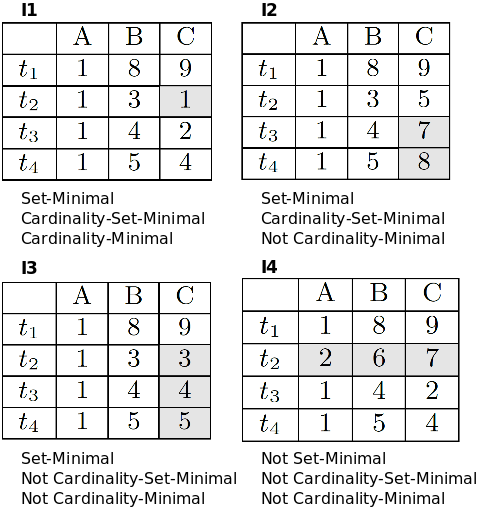
\includegraphics[scale=0.35]{cardinalityEg.png}
   \caption{Sample repairs from different repair space.}
   \label{fig:cardinalityEg}
\end{figure}


\section{Solution Overview} \label{sec:algo}
Finding minimal repairs has been shown to be NP-Complete even for FDs only \cite {Chiang}.
Moreover, finding minimal repairs for DCs and numerical values only is known to be MaxSNP-hard \cite{Bertossi}.
The work in \cite{XuChu} proposes an approximate holistic algorithm that is capable of generating nearly-optimal repairs for a given set of DCs.
The algorithm we propose for generating sapmle repairs for DCs is built upon two ideas: first, we try to generate a repair in a holistic manner as proposed in \cite{XuChu}, Second, we uses the
idea of generating random samples from the space of repairs, introduced in \cite{Beskales_sampling}.
Before going into the algorithm specifications, we will first see why the two of the above ideas cannot solve the problem alone.

\subsection{Previous Approaches}
First we will see why the repair sampling approach described in \cite{Beskales_sampling} is not self-sufficient to generate repairs for Denial-Constraints as well.
The idea in \cite{Beskales_sampling} is to grow the set of clean cells by merging the cells belonging to same equivalence class.
It is easy to build equivalence classes in case of FDs and CFDs, in other words when the set of predicates $B = \{ =, \neq\}$, 
but the equivalence class cannot be determined when the predicates are more loose, such as from set $B = \{ =, \neq\, <, >, \leq, \geq, \approx \}$.

Second, the approximate holistic algorithm in \cite{XuChu}, has two issues due to which it cannot be used for generating repairs.
One, the approximate algorithm uses minimum vertex cover (MVC) to find an approximately minimal repair, but it still does not gaurantee to cover all cardinality-Minimal space.
For example, consider the data instance given in  Table \ref{tab:eg1}, the MVC for the conflict hyper-edges is set $\{t_1.C, t_2.C and t_4.C\}$.
The holistic algorithm will pick one cell from MVC, say $t_2.C$ and form a frontier set and generate a repair expression for it.
The output repair from this will be the first repair in Table \ref{tab:eg2}, i.e. $t_1.C = t_2.C = t_3.C = t_4.C = 5$.
Although the cardinality-minimal repair is the second repair in Table \ref{tab:eg2}, i.e. $t_1.C = t_2.C = 3,t_4.D = V \leq 3$.
This cardinality-Minimal repair could have been acheived if the algorithm would have picked up cell $t_4.D$ first (that is not in MVC) and then $t_2.C$ to generate repair, we will show this in more detail in Section \ref{}.

The other issue with the holistic approach is that, it can also generate repairs which are not even Set-Minimal.
The cell modifications governed by the repair expression can generate new violations which are hendled in the next iteration of the algorithm.
We will see an example where a series of new violations can end up generating a Not Set-Minimal repair.
Consider a database instance and a set of DCs as shown in figure \ref{fig:eg4}.
The dotted box represents a violation hyperedge of a conflict hypergraph (CH).
The MVC for a single hyperedge CH can be any cell in that hyperedge.
Say, algorithm chose cell $t_2.B$ as MVC and generates a repair, as shown in Figure \ref{fig:notSetMinEg}(i), but introduces a new violation.
In the next iteration cell $t_2.A$ is a part of MVC and Figure \ref{fig:notSetMinEg}(ii) is the repair with a new violation, and so on, 
Figure \ref{fig:notSetMinEg}(i-iv) shows the repair and new violations introduced at each step of the iteration.
Figure \ref{fig:notSetMinEgFinal} shows all the cells changed in the repair process.
Now observe that the value of cell $t_2.B$ can be reverted back to its original value 5, and the resulting repair is shown in Figure \ref{fig:notSetMinEgOther} which is still a valid repair.
This proves that the holistic data cleaning algorithm can generate repairs which are not Set-Minimal.

\begin{figure}
   \centering
   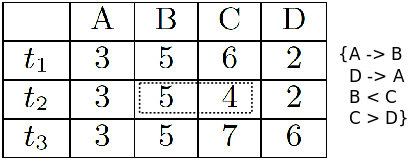
\includegraphics[scale=0.25]{eg4.png}
   \caption{Unclean database instance and a set of DCs. Dotted line is a hyperedge, showing violation.}
   \label{fig:eg4}
\end{figure}

\begin{figure}
   \centering
   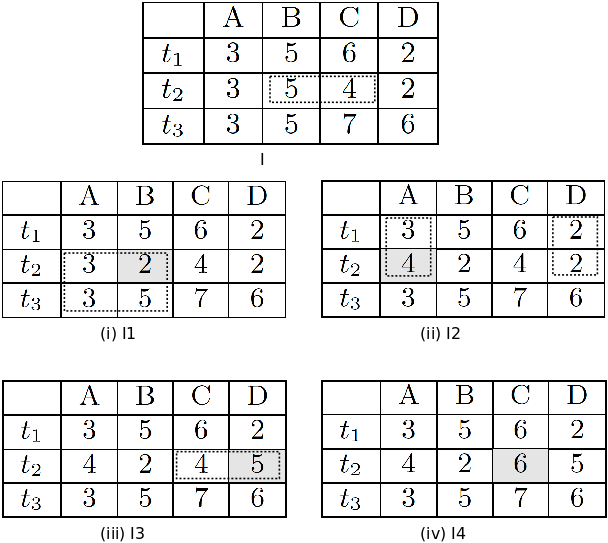
\includegraphics[scale=0.28]{notSetMinEg.png}
   \caption{Shows the repaired cell at each iteration and the new violation.}
   \label{fig:notSetMinEg}
\end{figure}

\begin{figure}
   \centering
   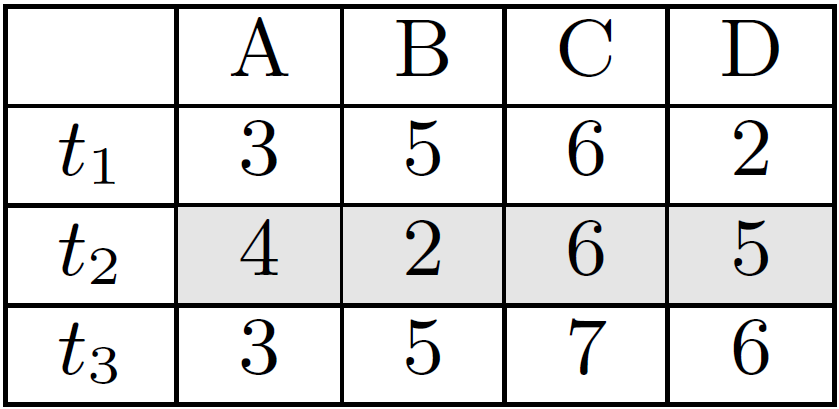
\includegraphics[scale=0.2]{notSetMinEgFinal.png}
   \caption{All the cell changed with respect to original I.}
   \label{fig:notSetMinEgFinal}
\end{figure}

\begin{figure}
   \centering
   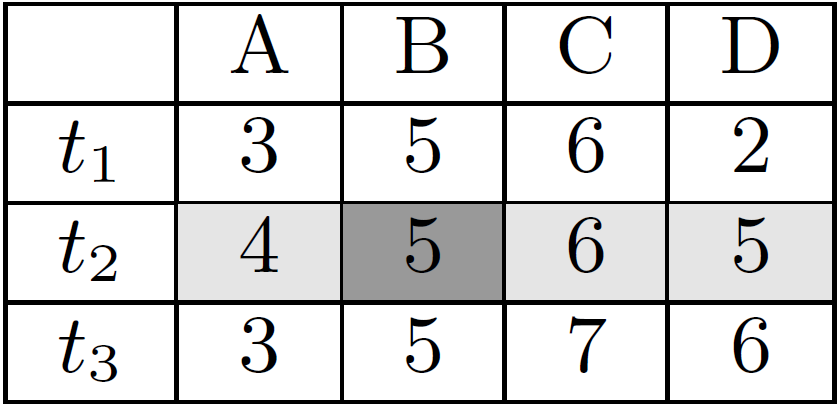
\includegraphics[scale=0.2]{notSetMinEgOther.png}
   \caption{Value of Cell $t_2.B$ can be reverted and the repair is still valid.}
   \label{fig:notSetMinEgOther}
\end{figure}

%
%\begin{table} \label{tab:eg1}
%\centering 
%\begin{tabular}{|c|c|c|c|c|}  \hline
%      & A & B & C & D 	\\ \hline
%   $t_1$ & 3 & 5 & 6 & 2 	\\ \hline
%   $t_2$ & 3 & 5 & 4 & 2 	\\ \hline
%   $t_3$ & 3 & 5 & 7 & 6 	\\ \hline
%\end{tabular}
%\caption{Sample Data.}
%\end{table}
%
%
%
%
%
%
%\begin{table} \label{tab:eg1}
%\centering 
%\begin{tabular}{|c|c|c|c|c|}  \hline
%      & A & B & C & D 	\\ \hline
%   $t_1$ & 3 & 5 & 6 & 2 	\\ \hline
%   $t_2$ & 3 & \cellcolor[gray]{0.9}2 & 4 & 2 	\\ \hline
%   $t_3$ & 3 & 5 & 7 & 6 	\\ \hline
%\end{tabular}
%\caption{Sample Data.}
%\end{table}
%
%\begin{table} \label{tab:eg1}
%\centering 
%\begin{tabular}{|c|c|c|c|c|}  \hline
%      & A & B & C & D 	\\ \hline
%   $t_1$ & 3 & 5 & 6 & 2 	\\ \hline
%   $t_2$ & \cellcolor[gray]{0.9}4 & 2 & 4 & 2 	\\ \hline
%   $t_3$ & 3 & 5 & 7 & 6 	\\ \hline
%\end{tabular}
%\caption{Sample Data.}
%\end{table}
%
%\begin{table} \label{tab:eg1}
%\centering 
%\begin{tabular}{|c|c|c|c|c|}  \hline
%      & A & B & C & D 	\\ \hline
%   $t_1$ & 3 & 5 & 6 & 2 	\\ \hline
%   $t_2$ & 4 & 2 & 4 & \cellcolor[gray]{0.9}5 	\\ \hline
%   $t_3$ & 3 & 5 & 7 & 6 	\\ \hline
%\end{tabular}
%\caption{Sample Data.}
%\end{table}
%
%\begin{table} \label{tab:eg1}
%\centering 
%\begin{tabular}{|c|c|c|c|c|}  \hline
%      & A & B & C & D 	\\ \hline
%   $t_1$ & 3 & 5 & 6 & 2 	\\ \hline
%   $t_2$ & 4 & 2 & \cellcolor[gray]{0.9}6 & 5 	\\ \hline
%   $t_3$ & 3 & 5 & 7 & 6 	\\ \hline
%\end{tabular}
%\caption{Sample Data.}
%\end{table}
%
%\begin{table} \label{tab:eg1}
%\centering 
%\begin{tabular}{|c|c|c|c|c|}  \hline
%      & A & B & C & D 	\\ \hline
%   $t_1$ & 3 & 5 & 6 & 2 	\\ \hline
%   $t_2$ & \cellcolor[gray]{0.9}4 & \cellcolor[gray]{0.9}2 & \cellcolor[gray]{0.9}6 & \cellcolor[gray]{0.9}5 	\\ \hline
%   $t_3$ & 3 & 5 & 7 & 6 	\\ \hline
%\end{tabular}
%\caption{Sample Data.}
%\end{table}
%
%\begin{table} \label{tab:eg1}
%\centering 
%\begin{tabular}{|c|c|c|c|c|}  \hline
%      & A & B & C & D 	\\ \hline
%   $t_1$ & 3 & 5 & 6 & 2 	\\ \hline
%   $t_2$ & \cellcolor[gray]{0.9}4 & \cellcolor[gray]{0.6}5 & \cellcolor[gray]{0.9}6 & \cellcolor[gray]{0.9}5 	\\ \hline
%   $t_3$ & 3 & 5 & 7 & 6 	\\ \hline
%\end{tabular}
%\caption{Sample Data.}
%\end{table}
%

\subsection{Algorithm Overview}
The algorithm we propose is inspired from the holistic data cleaning algorithm of \cite{XuChu}, with two major modifications.
One, we have introduced a randomness in selecting an hyperedge and a cell in an hyperedge, where as \cite{XuChu} used minimum vertex cover to select cells to start the repair.
Second, we have put constraints on which cells can be included in the frontier set. [MIGHT CHANGE -----]

We represent the violations in the database instance using hyperedges, similar to \cite{XuChu,Kolahi}.
After all the violations have been detected we get a set of hyperedges, and the graph induced by them is called a \textit{Conflict Hypergraph (CH)}.
It is an undirected hypergraph with a set of nodes P representing the cells and a set of annotated hyperedges E representing the relationships among cells violating a constraint.
More precisely, a \textit{hyperedge} is a set of violating cells from which one of them must change to repair the constraint, and contains: 
(a) the constraint $c$, which induced the conflict on the cells; (b) the list of nodes involved in the conflict.

Consider the example database instance given in Table \ref{tab:eg1} and the following set of DCs $\{ A \rightarrow C, B \rightarrow C, R[D=5] \rightarrow R[C=5], C \geq D \}$.
Figure \ref{fig:ch} represents a conflict hypergraph of the present state of the database violations w.r.t the given DCs.
Each hyperedge in the graph contains only the violating cells, and in order to repair it, at least one of its cells must get a new value.
We start our algorithm by picking an hyperedge at random and a random cell within that edge.
Algorithm assumes that this cell needs to be changed and hence identify all the other cells that are involved in the repair of this cell.
This starting set of newly identified cells is called \textit{frontier}.
We call \textit{repair expressions} the list of constant assignments and constraints among the frontier.
Similar to \cite{XuChu}, the frontier and the repair expressions form a \textit{Repair Context} (RC).
Once we are done with the repair context of the first chosen cell, we \textit{freeze} all the edges which got repaired using that RC.
By freeze, we mean that the cells belonging to those edges, if encountered in the frontier of any other RC later, cannot be changed.
If there are more edges remaining in the hypergraph, our algorithm again chooses a remaining hyperedge at random and chooses a non freezed cell from that edge,
and forms the RC for this new cell in the similar fashion.
The algorithm continues till there are no more hyperedges left in the graph.

For example, consider the DCs and hypergraph in Figure \ref{fig:ch}.
Lets say, the algorithm starts by choosing Edge $e4$ and cell $t_4[D]$.
The repair expression for this is simple, i.e. $t_4[D] \leq 3$, so we will assign it to a fresh value, call it $FV$ and cell $t_4[C]$ will be freezed.
Then we move onto choose the next edge, say this time we chose edge $e2$ and cell $t_2[C]$.
If we have to change $t_2[C]$ then the cell $t_3[C]$ in edge $e2$ should be changed, this gives us the expression $t_2[C] = t_3[C]$.
Cell $t_2[C]$ is related to edges $e1$ as well, and we get the expression $t_2[C] = t_1[C]$.
Cell $t_2[C]$ is related to edges $e4$ as well, and we get the expression $t_2[C] = t_4[C] = 3$, remember that cell $t_4[C]$ is frozen and cannot be changed.
The cell $t_1[C]$ is in edge $e5$ as well, hence the relation for cell $t_1[C]$ will be $t_1[C] \geq 3$.
Therefore the overall repair expression becomes $t_2[C] = t_1[C], t_2[C] = t_3[C], t_2[C] = t_4[C], t_4[C] = 3 and t_1[C] \geq 3$.
The cells and their new values will be: $t_2[C] = 3, t_1[C] = 3$ and $t_4[D] = FV$.

Notice that, the repair we obtained above is same as the second repair shown in Table \ref{tab:eg2}, which is ctually a Cardinality-Minimal repair.
This indicates that the randomized selection of cells is capable of generating Cardinality-Minimal repairs also.

\textbf{Proposition:} Randomized selection of cells gaurantee to cover Cardinality-Minimal repairs also. \\
\textit{Proof Sketch:} There are exponential possible repair expression in a CH depending upon the cells we start with.
Also, each repair expression has different satisfiability with different cardinality.
By using random selection we are allowing all the possible repair expressions, some of which will be Cardinality-Minimal.


\begin{figure}
   \centering
   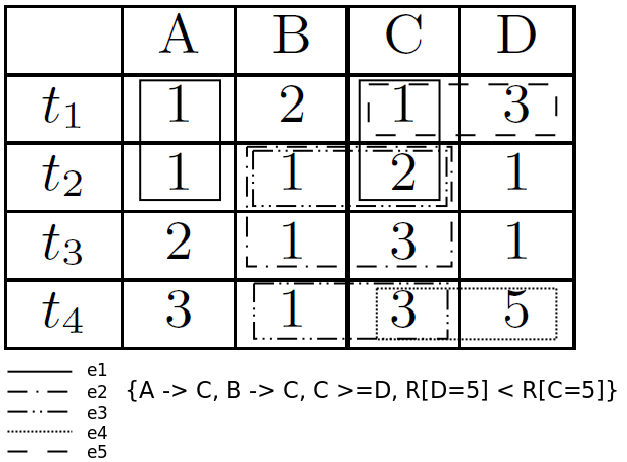
\includegraphics[scale=0.25]{ch.png}
   \caption{Conflict hypergraph.}
   \label{fig:ch}
\end{figure}



\balance

% The following two commands are all you need in the
% initial runs of your .tex file to
% produce the bibliography for the citations in your paper.
\bibliographystyle{abbrv}
\bibliography{project}  % vldb_sample.bib is the name of the Bibliography in this case
% You must have a proper ".bib" file
%  and remember to run:
% latex bibtex latex latex
% to resolve all references

\end{document}
